\chapter{Implementation}
\label{chap:implementation}
This chapter details the technical implementation of the ResNet-BiLSTM-Attention framework \autocite{Fischer2025ResNetBiLSTM} for validating SBDT in manufacturing environments. The implementation translates the conceptual framework described in \autoref{chap:methodology} into a functional system that processes manufacturing OCEL, extracts relevant features, trains models, and evaluates the fidelity of SBDT.

\section{Architecture and System Setup}

\subsection{Architecture}
The implementation follows a modular architecture. It can process both streams and batches of manufacturing data.

\begin{figure}[htbp]
  \centering
  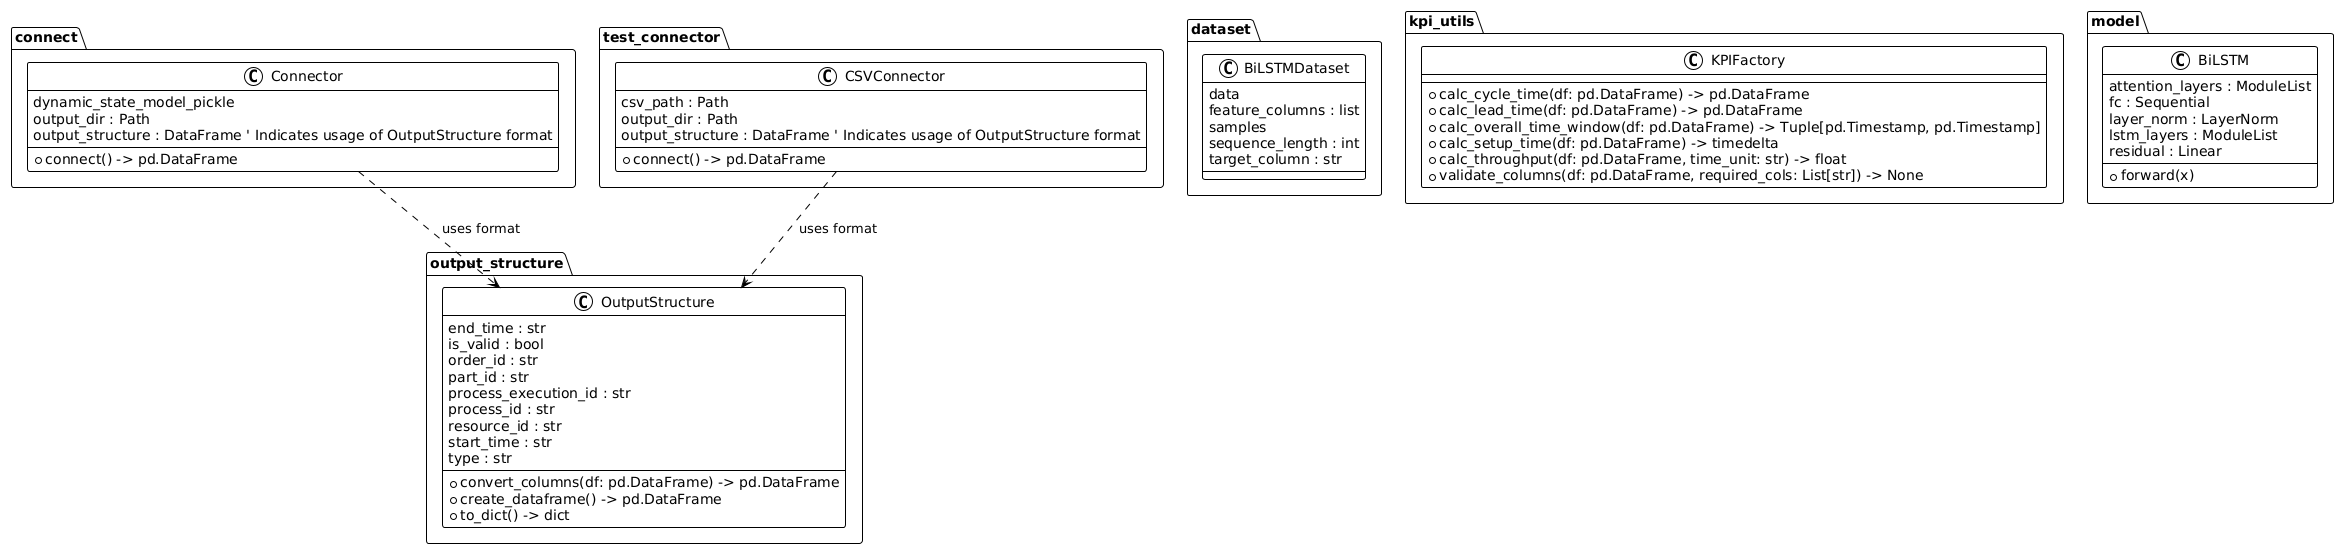
\includegraphics[width=0.8\textwidth]{figures/code.png}
  \caption{Unified Modelling Language (UML) model of the ResNet-BiLSTM-Attention framework for validating SBDT in manufacturing.environments.}
  \caption*{Source: Own figure.}
  \label{fig:DSR}
\end{figure}

The UML model \autocite{PlantUML} in \autoref{fig:DSR} illustrates the system's architecture, which consists of several components that interact to achieve the validation of SBDT. The components include:
\begin{itemize}
  \item \textbf{Data Connectors:} In the given code, two classes \texttt{InputStructure} and \texttt{OutputStructure} are responsible for reading and writing data. The \texttt{InputStructure} class reads raw data from the twin simulation, while the \texttt{OutputStructure} class writes the processed data into the OCEL format developed for this framework, see \autoref{label:sec:event_log_processing}. In this I/O model, the mapping logic is returned as well. The connector assigns IDs for different parts, resources, and processes. The IDs are used to identify the different components in the manufacturing process. This is a requirement for OCED. The mapping is returned as JSON files for each category, respectively.
  \item \textbf{KPIFactory:} Contains utility functions to calculate a diverse set of KPIs for PPC evaluation of the process.
  \item \textbf{Baseline Model:} Implements a baseline model for comparison with the ResNet-BiLSTM-Attention model. This model serves as a reference point to evaluate the performance of the more complex architecture.
  \item \textbf{Pytorch DataSet and DataLoader: BiLSTMDataset} Handles the conversion of raw data into a format suitable for the ResNet-BiLSTM-Attention model.
  \item \textbf{ResNet-BiLSTM-Attention:} The core model that combines ResNet and BiLSTM architectures with attention mechanisms to learn from the data.
\end{itemize}

\subsection{Tech Stack and Setup}
The implementation is built with Python 3.12 \autocite{Python}, using the following frameworks and libraries:

\begin{itemize}
  \item \textbf{PyTorch:} Powers the deep learning components, chosen for its dynamic computational graph that facilitates complex architecture development and debugging \autocite{PyTorch}.
  \item \textbf{Pandas \& NumPy:} Handle data manipulation, transformation, and numerical operations \autocite{NumPy, Pandas}.
  \item \textbf{Scikit-learn:} Provides implementation of the baseline model and evaluation metrics \autocite{ScikitLearn}.
  \item \textbf{Matplotlib \& Graphviz:} Generate visualizations of model architecture and performance \autocite{Matplotlib, Graphviz}.
  \item \textbf{UV Package Manager:} Ensures reproducible dependency management with exact version pinning \autocite{UV}.
\end{itemize}

Besides well established SOTA packages, PyTorch was preferred over TensorFlow due to its flexibility and ease of use, especially for research purposes. The implementation is designed to be modular and extensible, allowing for future enhancements and adaptations to different manufacturing environments.
The system is designed to run on a standard workstation with a multi-core CPU and an optional GPU for accelerated training. The given framework utilizes CUDA \autocite{NVIDIA_CUDA} for GPU acceleration, which significantly speeds up the training process. The system is capable of processing large datasets efficiently, making it suitable for real-time applications in manufacturing environments.


\section{Data Preprocessing}
\label{sec:event_log_processing}

After laying out the architecture and system setup, this section focuses on the data preprocessing steps necessary for preparing the input data for the baseline modelResNet-BiLSTM-Attention model.


\subsection{OCEL Format}

Both models used in this thesis require the input data to be in the OCEL format, see \autoref{sec:object-centric-event-logs}. The columns are inspired by the twin comparison model by \autocite{schwede2024learning}. For the given framework, the format is expected as input in the following format:

\begin{table}[htbp]
  \centering
  \caption{Detailed structure, data types, and description of the processed manufacturing OCEL.}
  \label{tab:output_structure_detailed}
  % Adjust the width 'p{6cm}' of the description column as needed, or use tabularx
  \begin{tabular}{l l p{6cm}} % l=left-aligned, p{width}=paragraph column
    \toprule
    \textbf{Column Name}            & \textbf{Data Type}       & \textbf{Description}                                                                                                                              \\
    \midrule
    \texttt{process\_execution\_id} & \texttt{int}             & Unique identifier for the specific process recorded.                                                                                              \\
    \texttt{order\_id}              & \texttt{Index (int/str)} & Identifier for the overall manufacturing order this event belongs to.                                                                             \\
    \texttt{start\_time}            & \texttt{Timestamp [UTC]} & The precise timestamp marking the beginning of the event, adjusted to UTC.                                                                        \\
    \texttt{end\_time}              & \texttt{Timestamp [UTC]} & The precise timestamp marking the end of the event, adjusted to UTC.                                                                              \\
    \texttt{duration}               & \texttt{float} (seconds) & The calculated duration of the event (\texttt{end\_time} - \texttt{start\_time}) in total seconds.                                                \\
    \texttt{part\_id}               & \texttt{int}             & Identifier for the specific part or component being processed or handled during the event.                                                        \\
    \texttt{resource\_id}           & \texttt{int}             & Identifier for the machine, station, or other resource involved in the event.                                                                     \\
    \texttt{process\_id}            & \texttt{int}             & Identifier indicating the type of process step or operation performed (e.g., milling, assembly).                                                  \\
    \texttt{type}                   & \texttt{str}             & A textual description or category classifying the type of event recorded.                                                                         \\
    \texttt{is\_valid}              & \texttt{bool}            & Boolean flag indicating whether the recorded event sequence or outcome is considered valid (e.g., based on model prediction or predefined rules). \\
    \bottomrule
  \end{tabular}
\end{table}

The terms are consistent with the upper cited framework. For the model components, following features may be considered:

\begin{enumerate}
  \item \textbf{Time Model:}
        \\ Features: \texttt{duration}, \texttt{start\_time}, \texttt{end\_time} and further engineered features, see \autoref{sec:feature_engineering}.

  \item \textbf{Transition Model:}
        \\ Features: \texttt{process\_id}, \texttt{resource\_id}, \texttt{end\_time}.

  \item \textbf{Transformation Model:} Features related to the object undergoing transformation.
        \\ Features: \texttt{part\_id}.

  \item \textbf{Quality Model:} Status regarding quality-specific features.
        \\ Status: Exclusion of quality information in the given model.

  \item \textbf{Resource Model:} Features characterizing the resource state or involvement.
        \\ Features: \texttt{resource\_id}, \texttt{process\_id}, \texttt{part\_id}.

  \item \textbf{Resource Capacity Model:} Status related to resource capacity modeling.
        \\ Features: \texttt{resource\_id}; Note: Insufficient data available for detailed capacity modeling.

  \item \textbf{Process Model:} Features describing the overall state of the process execution.
        \\ Features: \texttt{process\_id}, \texttt{part\_id}, \texttt{resource\_id}.
\end{enumerate}

The table shown is the least required structure for the OCEL format. Other columns will be added situationally \autoref{chap:case-study}. The \texttt{process\_execution\_id} is a unique identifier for each event, while the \texttt{order\_id} serves as the index for the order, similar to a case ID. The \texttt{start\_time} and \texttt{end\_time} columns are in UTC format, and the duration is calculated in seconds. The \texttt{part\_id}, \texttt{resource\_id}, and \texttt{process\_id} columns provide identifiers for the part, resource, and process type, respectively. The \texttt{type} column contains a textual description of the event, part or other information. The modeller can decide how to use the \texttt{type} column. The last \texttt{is\_valid} column indicates whether the event sequence is valid.

This table does not forbid adding relational logic by the modeller. For example, each ID may be a foreign key to another table. Each row in the OCEL represents a single event instance. This schema aligns with OCED principles (\autoref{sec:object-centric-event-logs}) by explicitly linking each recorded event instance (\texttt{process\_execution\_id} per timestamp) to the multiple object instances (\texttt{order\_id}, \texttt{part\_id}, \texttt{resource\_id}, \texttt{process\_id}) involved in its execution. This inherent multi-object relationship within each event record is important for modelling complex process dependencies. The structure empowers the representation of complex control flows often found in manufacturing. Parallel execution paths (AND-split) can be inferred by identifying events associated with different resources or process steps occurring \textit{within} overlapping time intervals (\texttt{start\_time}, \texttt{end\_time}) but related to shared object instances, such as a common \texttt{order\_id}. Alternative paths and process variants (EXCLUSIVE OR-split) are explicitly captured through the diversity of event sequences observed across different process instantiations (e.g., grouped by \texttt{order\_id}); the log records exactly which path or sequence of activities occurred for each instance. The object-centric nature enriches this analysis by providing context (e.g., the specific \texttt{part\_id} or \texttt{resource\_id} involved) that can explain why a particular variant or choice was executed. The OCEL retains its sequential lineral character by grouping it by \texttt{order\_id} and sorting ascending related to \texttt{end\_time}. This allows for the reconstruction of the process flow.

Because conciseness of the data structure was a requirement a priori, the OCEL format is not fully compliant with the OCED standard \autocite{van2023object}. The OCEL format used in this thesis is a rather simplified. Specifically, this simplification means the schema does not include distinct tables for object instances and their types, explicit modelling of static O2O relationships or the capability to store timestamped attributes associated directly with objects rather than events. Despite these omissions the implemented structure retains the core OCED principles. The goal is rather to \textit{learn} these relationships from the data itself.
% Data preparation and transformation
% Feature engineering for order reconstruction (→ reference to 3.2)
% Techniques for data partitioning
% Implementation of the process mining concepts (→ reference to 2.3)

\section{Model Implementation}

\subsection{Whitebox Baseline Model}
As a baseline model, a whitebox model is implemented to provide a reference point for the performance of the ResNet-BiLSTM-Attention model. The whitebox model is based on a simple decision tree classifier, which is interpretable and easy to understand. This model serves as a benchmark for evaluating the performance of the more complex ResNet-BiLSTM-Attention model. For the concrete implementation, the \texttt{DecisionTreeClassifier} from the \texttt{sklearn.tree} module is used. The decision tree classifier is trained on the same dataset as the ResNet-BiLSTM-Attention model, and its performance is compared using various metrics such as accuracy, precision, recall, and F1-score.


% Selection and implementation of classification algorithms (→ reference to 4.3)
% Training, validation, and model evaluation
% Technical realization of the ML-based V\&V approach (→ reference to 3.3)
\subsection{ResNet BiLSTM Multi-Head Self-Attention Network}
As a challenger model, the ResNet-BiLSTM-Attention model is implemented, see \autoref{sec:bilstm}. This model combines the strengths of residual networks (ResNet) and bidirectional long short-term memory networks (BiLSTM) with multi-head self-attention mechanisms. The model is implemented using the PyTorch modules \texttt{torch.nn}, \texttt{torch.functional} and \texttt{torch.optim} \autocite{PyTorch}.

\begin{figure}[htbp]
  \centering
  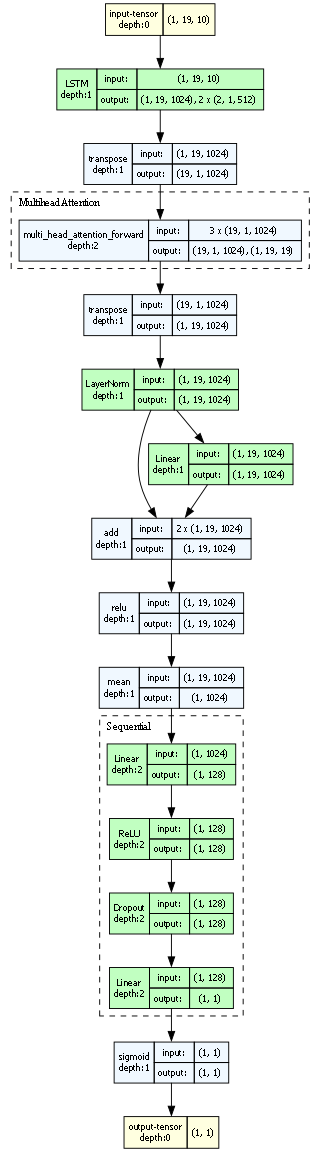
\includegraphics[width=0.8\textwidth]{figures/architecture.png}
  \caption{ResNet-BiLSTM-Attention architecture. The model consists of a ResNet block, followed by a BiLSTM layer and a multi-head self-attention mechanism. The output is then passed through a fully connected layer for classification.}
  \label{fig:DSR}
  \caption*{Source: Own Torchview illustration.}
\end{figure}


\section{Model Evaluation}
% cite evaluation metrics
% Evaluation metrics for classification tasks (→ reference to 3.4)


\subsection{Processing Batch Data}


\subsection{Processing Stream Data}
% Describe helper functions here